\chapter{Implementazione}
\label{cha:implementazione}

In questo capitolo viene mostrata l'implementazione della pipeline dati sviluppata durante
il tirocinio. Dopo aver descritto il contesto e le tecnologie adottate nei capitoli precedenti, qui l’attenzione si sposta sugli aspetti pratici della realizzazione.
L’obiettivo principale è stato quello di trasformare un unico script monolitico in un sistema modulare e automatizzato, basato su Apache Airflow e containerizzato tramite Docker. La nuova architettura non solo consente di programmare e monitorare l’esecuzione dei workflow, ma integra anche strumenti di osservabilità, rendendo possibile analizzare in tempo reale lo stato delle esecuzioni e le risorse utilizzate.

Nel corso del capitolo verranno quindi analizzati:


\begin{itemize}
    \item la definizione del DAG in Airflow e l’adattamento degli script esistenti a PostgreSQL, con esempi di refactoring effettuati durante il lavoro;
    \item la containerizzazione del sistema, descrivendo nel dettaglio il Dockerfile e il file docker-compose.yml;
    \item l’infrastruttura di monitoraggio, con le configurazioni di StatsD, Prometheus e Grafana;
    \item l’integrazione dei diversi componenti e le modalità di deploy dell’applicazione.
\end{itemize}

In questo modo si vuole mostrare il percorso seguito per passare da una soluzione monolitica e difficile da mantenere a un’infrastruttura completa, affidabile, automatizzata e osservabile.

\begin{figure}[h]
    \centering
    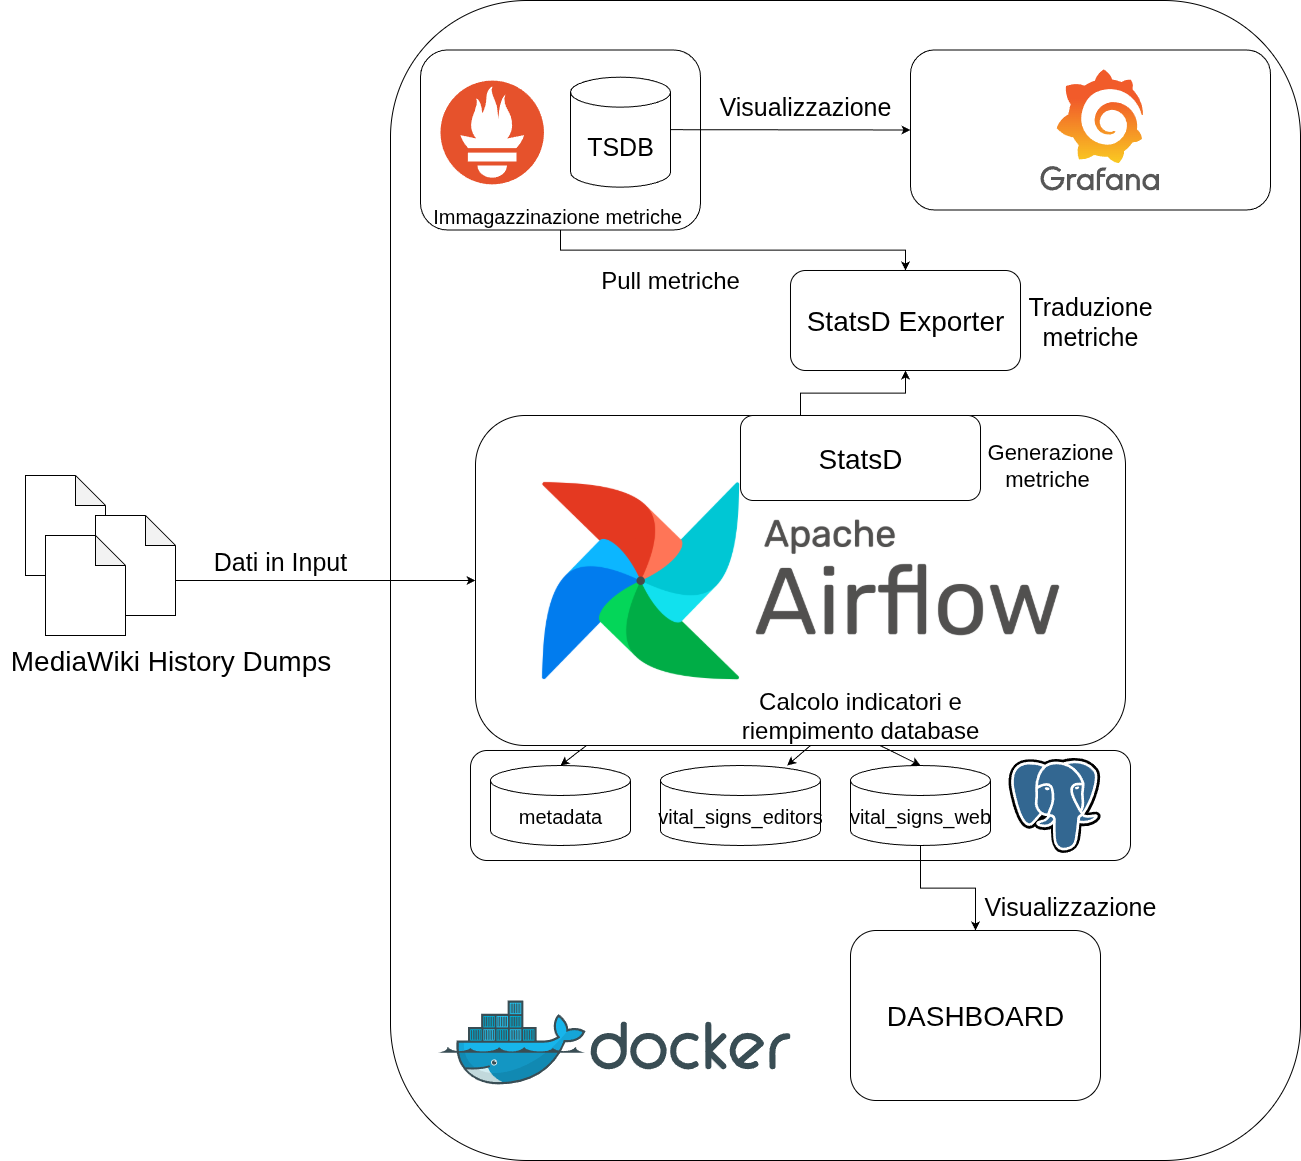
\includegraphics[width=\textwidth]{img/vital-signs-pipeline.drawio.png}
    \caption{Schema logico dell'architettura del sistema}
    \label{fig:architettura_sistema}
\end{figure}

\section{DAG e script}
\label{sec:dag_script}

Come introdotto nella Sezione~\ref{sec:airflow}, il Directed Acyclic Graph (DAG) è lo strumento con cui Apache Airflow permette di modellare un workflow come un insieme di task con relazioni di dipendenza.

Nel progetto ho definito il DAG vital\_signs, contenuto nel file vital\_signs\_dag.py all’interno della cartella dags/. Questo DAG ha il compito di processare i dati provenienti dai MediaWiki History Dumps, eseguendo diversi calcoli su di essi e popolando progressivamente due database distinti: prima quello degli editors, che raccoglie le metriche derivate dai dump, e successivamente quello web, in cui vengono calcolati e salvati i vital signs a partire dalle metriche estratte.

Vediamo ora come è stato definito il DAG, le sue caratteristiche principali e come sono stati adattati gli script esistenti per funzionare in questo nuovo contesto.

\newpage

\begin{lstlisting}[language=Python, caption=Definizione del DAG in Airflow, label=lst:dag_definition]
# Import delle librerie necessarie e funzioni di supporto
with DAG(
    dag_id='vital_signs',
    default_args={
        'owner': 'andrea_denina',
        'depends_on_past': False,
        'start_date': datetime(2025, 4, 15),
        'retries': 1,
        'retry_delay': timedelta(minutes=5),
    },
    description='Compute Community Health Metrics (CHM) 
    from MediaWiki History dumps for multiple languages',
    schedule_interval='0 0 10 * *',
    catchup=False,
    max_active_runs=1
) as dag:
    # Definizione dei task
\end{lstlisting}

Il codice in lst. \ref{lst:dag_definition} mostra la definizione del DAG vital\_signs e i suoi parametri principali.

In particolare:

\begin{itemize}
    \item \textbf{dag\_id}: assegna un identificativo univoco al DAG, in questo caso vital\_signs.
    \item \textbf{default\_args}: raccoglie i parametri comuni a tutte le task, come l'owner, la data di inizio, il numero di retry e il ritardo tra un tentativo e l'altro.
    \item \textbf{start\_date}: definisce la data a partire dalla quale Airflow può schedulare le esecuzioni del DAG.
    \item \textbf{schedule\_interval}: stabilisce la frequenza di esecuzione. È stata scelta un'espressione cron che fa partire il DAG ogni 10 del mese, in linea con le tempistiche di pubblicazione dei dump.
    \item \textbf{catchup}: impostato a False, evita che al primo avvio il DAG tenti di recuperare retroattivamente tutte le esecuzioni mancate dal start\_date.
    \item \textbf{max\_active\_runs}: limita il numero di esecuzioni contemporanee del DAG a uno, per prevenire conflitti nell'accesso ai dati.
\end{itemize}


\subsection{Struttura delle task}
\label{subsec:struttura_task}

Nel DAG vital\_signs le task sono tutte implementate come PythonOperator,
quindi ciascuna invoca uno script Python specifico.
La pipeline è delimitata da due sentinelle logiche, start ed end (entrambi EmptyOperator), fra le quali si sviluppa il flusso di elaborazione.
Subito dopo l’avvio, la task create\_dbs prepara l’ambiente applicativo creando e inizializzando le tabelle dei due database coinvolti (editors e web).
A questo punto il DAG si ramifica per lingua (in base a wikilanguagecodes) e per ogni edizione linguistica vengono eseguiti in sequenza tre step: 
<code>\_process\_dump per estrarre e caricare le metriche dai MediaWiki History Dumps nel DB degli editor,
<code>\_calc\_flags per calcolare i flag/profili degli editor,
<code>\_calc\_streaks per derivare le streak di attività.

Terminata la fase per lingua sul database vital\_signs\_editors, una fase cross wiki (calc\_primary\_language) calcola la lingua primaria degli utenti a partire dalle metriche calcolate nelle precedenti fasi.
Infine, avviene una seconda ramificazione per lingua dove, con <code>\_calc\_vs, si computano i vital signs e si popolano le tabelle del database  vital\_signs\_web a partire dalle metriche già consolidate.
L’intera catena è vincolata da dipendenze esplicite (>>) che assicurano l’ordine corretto; inoltre, ogni task utilizza callback di logging di esito (on\_success\_callback, on\_failure\_callback) per tracciare in modo uniforme completamenti e fallimenti delle esecuzioni.
In questo modo il DAG rimane leggibile e modulare: ogni task incapsula un passaggio ben definito e l’orchestrazione di Airflow garantisce una progressione deterministica dall’ingestione dei dump fino alla produzione dei vital signs.


\begin{lstlisting}[language=Python, caption={Esempio di definizione di una task e dipendenze del DAG}, label=lst:dag_tasks]
start = EmptyOperator(task_id='start', dag=dag)
end = EmptyOperator(task_id='end', dag=dag)

create_dbs_task = PythonOperator(
    task_id="create_dbs",
    python_callable=create_db,
    dag=dag,
    op_args=[wikilanguagecodes],
    on_success_callback=log_task_end,
    on_failure_callback=log_task_failure,
)

...

start >> create_dbs_task >> editors_db_group \
      >> primary_language_task >> web_db_group >> end
\end{lstlisting}

Nel codice in lst. \ref{lst:dag_tasks} è mostrato un esempio di definizione di una task (create\_dbs) e la struttura delle dipendenze del DAG.
Come si può notare la task chiama la funzione create\_db, definita in un file nella cartella scripts/ e importata come una libreria.


\clearpage